\begin{figure}[htbp]
\centering
\begin{minipage}[t]{0.49\textwidth}
\centering
\begin{adjustbox}{width=1.0\textwidth}
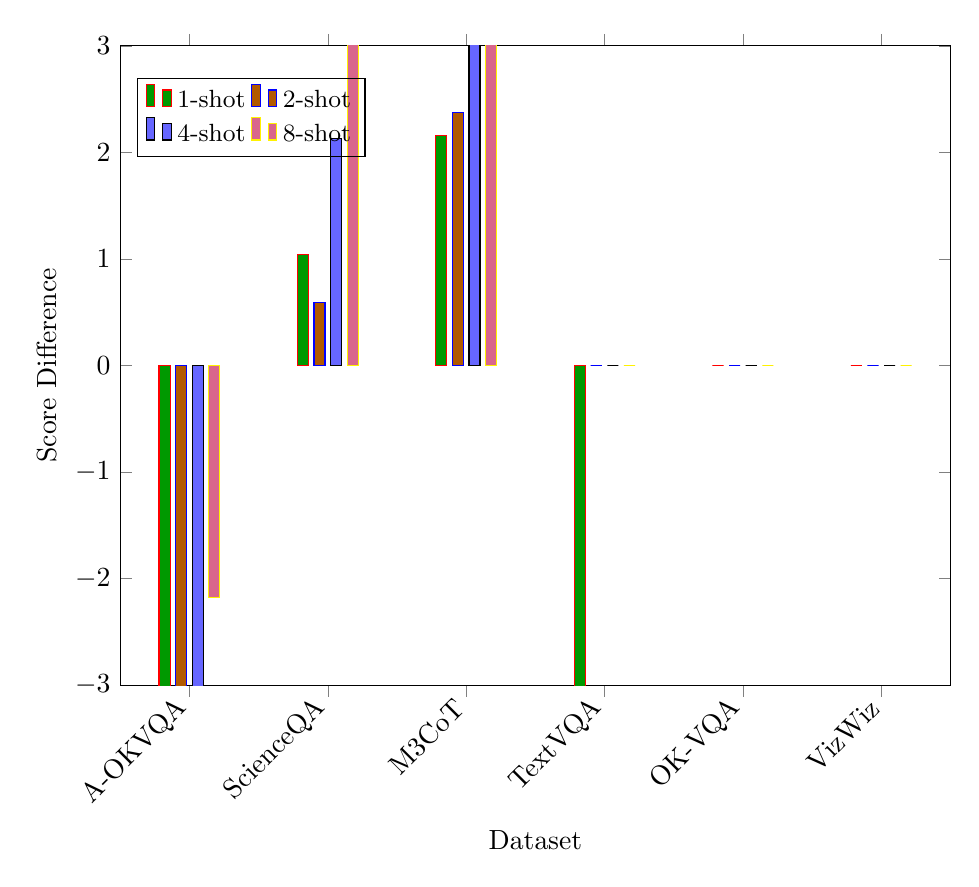
\begin{tikzpicture}
\begin{axis}[
    ybar,
    bar width=4pt,
    width=\textwidth,
    height=0.8\textwidth,
    enlarge x limits=0.1,
    ylabel={Score Difference},
    xlabel={Dataset},
    xtick=data,
    xticklabel style={rotate=45, anchor=east},
    symbolic x coords={A-OKVQA, ScienceQA, M3CoT, TextVQA, OK-VQA, VizWiz},
    ymin=-3, ymax=3,
    legend style={
        at={(0.02,0.95)},
        anchor=north west,
        fill=none,
        legend columns=2,
        font=\small
    },
    legend cell align={left},
    cycle list name=color list,
]
\addplot+[fill=green!60!black] coordinates { (A-OKVQA, -5.68) (ScienceQA, 1.04) (M3CoT, 2.16) (TextVQA, -11.42) (OK-VQA, 0.00) (VizWiz, 0.00) };
\addplot+[fill=orange!70!black] coordinates { (A-OKVQA, -5.33) (ScienceQA, 0.59) (M3CoT, 2.37) (TextVQA, 0.00) (OK-VQA, 0.00) (VizWiz, 0.00) };
\addplot+[fill=blue!60] coordinates { (A-OKVQA, -4.02) (ScienceQA, 2.13) (M3CoT, 6.04) (TextVQA, 0.00) (OK-VQA, 0.00) (VizWiz, 0.00) };
\addplot+[fill=purple!60] coordinates { (A-OKVQA, -2.18) (ScienceQA, 3.57) (M3CoT, 4.87) (TextVQA, 0.00) (OK-VQA, 0.00) (VizWiz, 0.00) };
\legend{1-shot, 2-shot, 4-shot, 8-shot}
\end{axis}
\end{tikzpicture}
\end{adjustbox}
\caption*{(a) JICES vs. Random Sampling (Llama-3.2-11B-Vision-Instruct)}
\end{minipage}
\hfill
\begin{minipage}[t]{0.49\textwidth}
\centering
\begin{adjustbox}{width=1.0\textwidth}
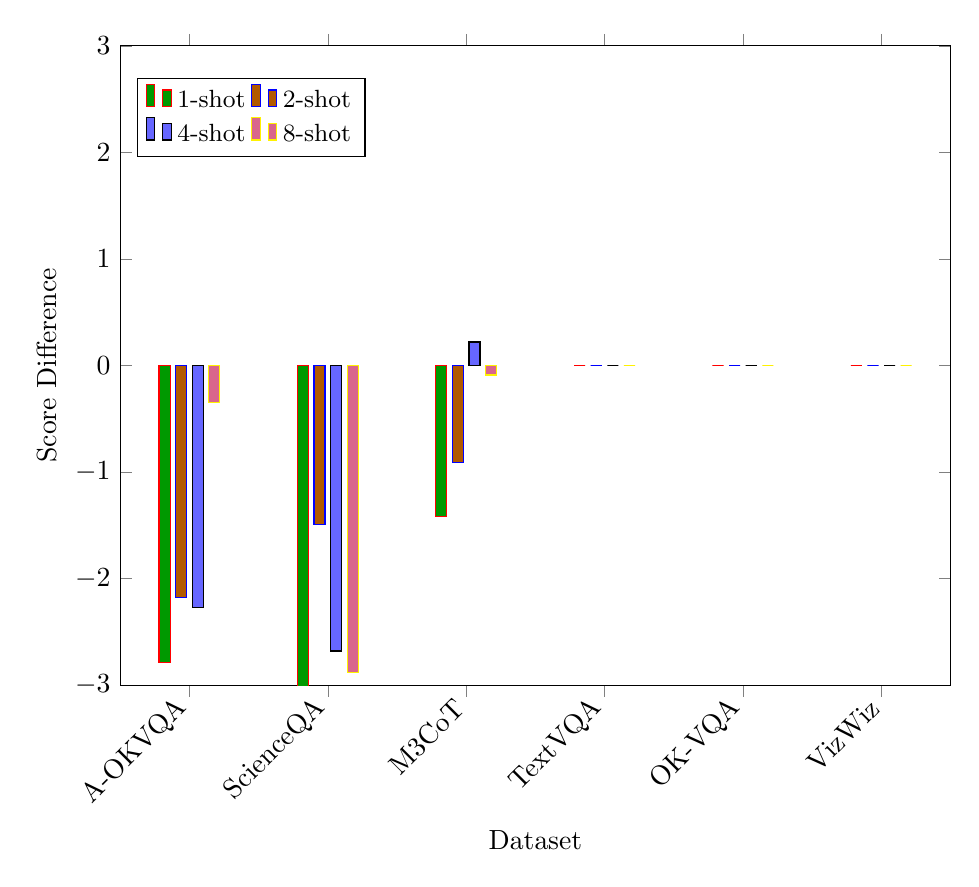
\begin{tikzpicture}
\begin{axis}[
    ybar,
    bar width=4pt,
    width=\textwidth,
    height=0.8\textwidth,
    enlarge x limits=0.1,
    ylabel={Score Difference},
    xlabel={Dataset},
    xtick=data,
    xticklabel style={rotate=45, anchor=east},
    symbolic x coords={A-OKVQA, ScienceQA, M3CoT, TextVQA, OK-VQA, VizWiz},
    ymin=-3, ymax=3,
    legend style={
        at={(0.02,0.95)},
        anchor=north west,
        fill=none,
        legend columns=2,
        font=\small
    },
    legend cell align={left},
    cycle list name=color list,
]
\addplot+[fill=green!60!black] coordinates { (A-OKVQA, -2.79) (ScienceQA, -3.72) (M3CoT, -1.42) (TextVQA, 0.00) (OK-VQA, 0.00) (VizWiz, 0.00) };
\addplot+[fill=orange!70!black] coordinates { (A-OKVQA, -2.18) (ScienceQA, -1.49) (M3CoT, -0.91) (TextVQA, 0.00) (OK-VQA, 0.00) (VizWiz, 0.00) };
\addplot+[fill=blue!60] coordinates { (A-OKVQA, -2.27) (ScienceQA, -2.68) (M3CoT, 0.22) (TextVQA, 0.00) (OK-VQA, 0.00) (VizWiz, 0.00) };
\addplot+[fill=purple!60] coordinates { (A-OKVQA, -0.35) (ScienceQA, -2.88) (M3CoT, -0.09) (TextVQA, 0.00) (OK-VQA, 0.00) (VizWiz, 0.00) };
\legend{1-shot, 2-shot, 4-shot, 8-shot}
\end{axis}
\end{tikzpicture}
\end{adjustbox}
\caption*{(b) JICES vs. Random Sampling (LLaVA-CoT)}
\end{minipage}
\caption{Comparison of JICES vs. Random Sampling on 6 vision-language datasets.}
\label{fig:jices-two-plots-trimmed}
\end{figure}